% ============================================== %
%
% Methodology.tex
%
%% ============================================== %
\chapter{Methodology} \label{chap:methodology}
\hypersetup{colorlinks=true, linkcolor=red}
    In this chapter, the methodology used to split the data and train the models is presented. In addition, the fundamental concepts behind the models used are explained.
    \section{Overview of Models Analyzed}
        In this comparative study a total of ten popular models are selected for analysis of their perfomance on Kinect-based data.
        \subsection{Scikit-Learn}  

            Scikit-Learn is a Python library designed for Machine Learning, it offers a wide range of \textit{state of the art} algorithms for medium scale supervised and unsupervised problems. It emphasizes ease of use, perfomance, and API consistency, targeting non specialists with its high level approach. It stands out for its minimal dependecies and broad accessibility, being distributed under the simplified BSD license. It integrates well with the Python ecosystem, making it highly desirable for both academic and commercial applications \cite{scikit-learn}.

        \subsection{Models Selection}

        The models presented in Table \ref{tab:movements_table} are used for the classification task. Selected on a basis of popularity and performance, these models are widely used in the machine learning community. The models are implemented using the \textit{scikit-learn} library and it's functions for training, testing and evaluating\cite{sklearn_api}. 

        \begin{table}[ht]
            \centering
            \begin{tabular}{@{}clcl@{}}
                \toprule
                \multicolumn{4}{c}{\textbf{Model Name}} \\
                \midrule
                1 & Support Vector Machine & 6 & Linear Discriminant Analysis \\
                2 & Gaussian Naive Bayes & 7 & Multi-Layer Perceptron \\
                3 & Random Forest & 8 & K-Nearest Neighbors \\
                4 & Gradient Boosting & 9 & AdaBoost \\
                5 & Logistic Regression & 10 & Decision Tree \\
                \bottomrule
            \end{tabular}
            \caption{Models selected for use in this thesis.}
            \label{tab:movements_table}
        \end{table}
    \newpage
    
    \section{Analysis of Top-Performing Models}
        In this section the models that performed best in the Chapter \ref{chap:results_and_discussion} are analyzed. The models are analyzed in terms of their implementation.

        \subsection{Random Forest}
           Also known as \textit{random decision forests}, is a method of ensemble learning used for classification, regression, and various other tasks. It involves building numerous decision tress during the training phase. In classification tasks, the class chosen by the majority of trees is the output of the random forest \cite{ho_random_1998}.

           \begin{figure}[H]
            \centering
            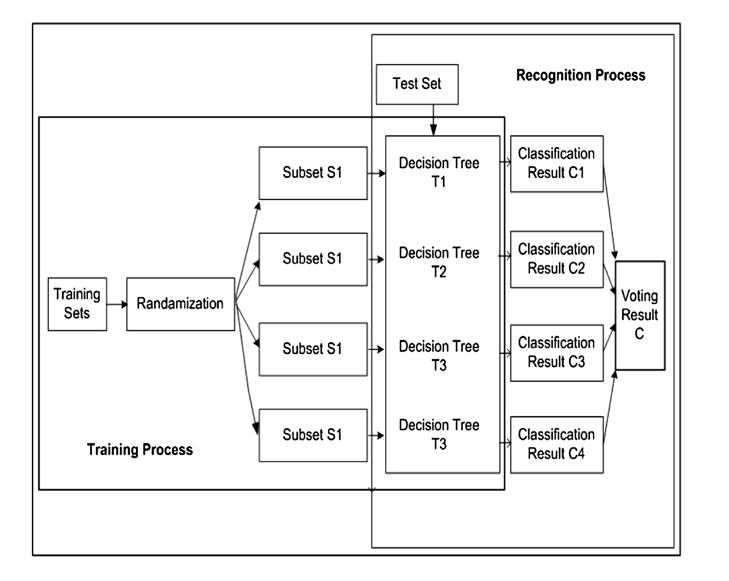
\includegraphics[width=.7\textwidth]{../src/resources/rf_image.png}
            \caption{
                Random Forest Classifier architecture \cite{parmar_review_2019}.
            }
            \label{fig:random_forest}
            \end{figure}

            The main steps involved in building a random forest classifier are as follows:
           
            \begin{enumerate}
                \item Define $M$ as the number of features in each subset.
                \item Randomly select a feature subset $\theta_k$ from the full set, distinct from proceding subset $\theta_{1},..., \theta_{k-1}$.
                \item Train decision trees on each $\theta_k$ denoted as $h(X, \theta_k)$.
                \item Iteratively select new $\theta_k$ subsets and train untill all tress are built.
                \item Classify test data by majority vote of all trees in the forest.
            \end{enumerate}

            Random forests consist of numerous decision trees. Randomization in tree building—through sampling instances and feature subsets via bagging—enhances diversity, reducing overfitting and improving generalization. Feature subsets $\theta_k$​ are chosen by bagging, and the importance of features is ranked by their impact on the model's accuracy. The "strength" and "correlation" of the forest are influenced by $M$, with optimal values providing a balance. The random forest's efficiency is due to its parallel structure, accelerating classification significantly \cite{parmar_review_2019}.
            
        \subsection{Gradient Boosting}
            Gradient boosting is a machine learning method that refines predictions iteratively, combining the strengths of simple models, like decision trees, into a more accurate ensemble. Each iteration, represented by $F_m(x)$, improves upon the last by adding a weighted decision tree $\rho_m h_m(x)$ that addresses the previous errors. The process follows the \textit{principle of gradient descent}, where $h_m(x)$ is trained to predict the negative gradient of the loss function, effectively reducin the residual between the predicted and true values. The ensemble begins with a single model $F_0(x)$, which is updated by the formula:
            \begin{equation}
                F_m(x) = F_{m-1}(x) + \rho_m h_m(x)
            \end{equation}
            The aim is to minimize the loss function $L(y, F_m(x))$ at each step, ensuring the model's prediction become progressively more accurate \cite{bentejac_comparative_2021}.
            \begin{figure}[H]
                \centering
                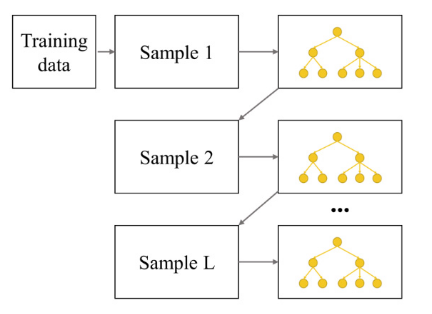
\includegraphics[width=.5\textwidth]{../src/resources/boosting.png}
                \caption{
                    Gradient Boosting Classifier architecture \cite{cha_comparison_2021}.
                }
                \label{fig:gradient_boosting}
            \end{figure}
        \subsection{Logistic Regression}
            Logistic Regression is a statistical method used for binary classification. It predicts the probability of a binary outcome based on one or more predictor variables. 

            \begin{figure}[H]
                \centering
                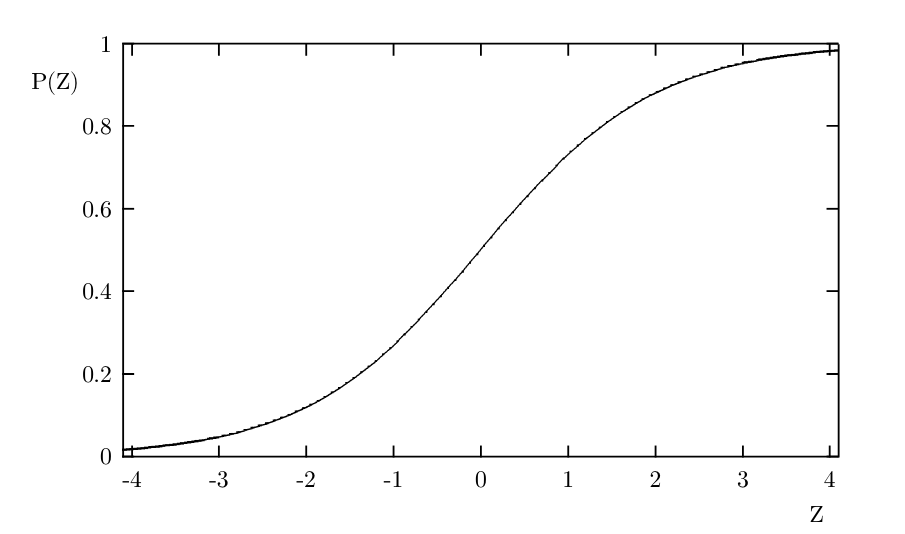
\includegraphics[width=.6\textwidth]{../src/resources/logistic.png}
                \caption{
                    Logistic curve P(Z) \cite{cramer_origins_2002}.
                }
                \label{fig:logistic_regression}
            \end{figure}
        \subsection{Linear-Discriminant Analysis}
            Linear Discriminant Analysis (LDA) is a method used in statistics and machine learning to find a linear combination of features that separates two or more classes of objects or events. It does so by maximizing the ratio of between-class variance to the within-class variance in any particular data set, thereby ensuring maximum separability.

            In the binary class, the goal is to find a linear combination $w$ tjat separates the classes. This involves computing the mean vectors $m_1$ and $m_2$ for each class, the within class scatter matrix $S_W$, and the between class scatter amtix $S_B$. The linear discriminants are then the eigenvectors of $S_W^{-1}S_B$. 

            \begin{figure}[H]
                \centering
                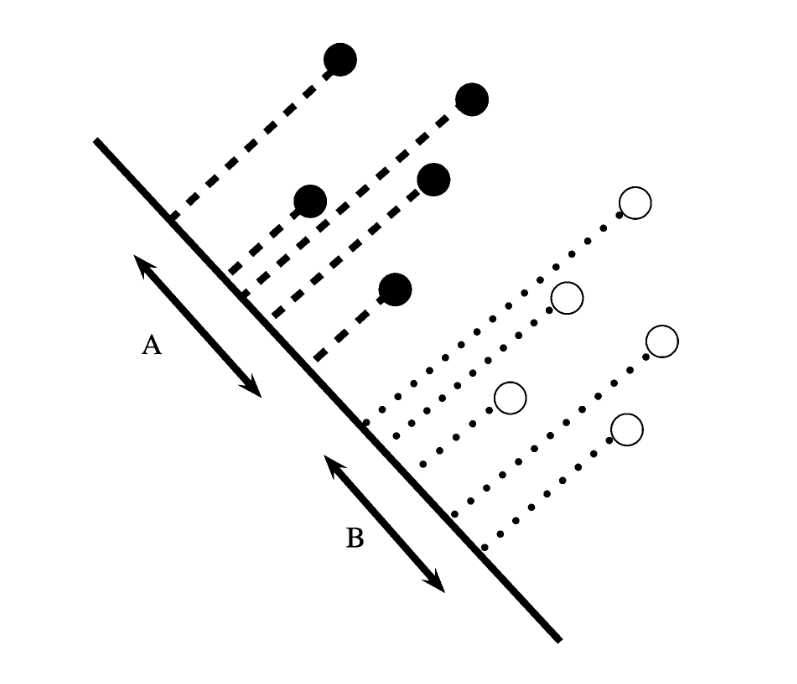
\includegraphics[width=.6\textwidth]{../src/resources/lda.png}
                \caption{
                    Linear Discriminant Analysis \cite{xanthopoulos_linear_2013}.
                }
                \label{fig:linear_discriminant_analysis}
            \end{figure}

            For multi class problems, the same principle applies but extends to multiple classes. The within class scatter matrix $S_W$ and between class scatter matrix $S_B$ are computed considering all classes, and the objective is to find the linear discriminants that maximize the separation among all classes.  

            The simplicity and effectiveness of LDA, especially under the assumptions of normality and equal class covariances, make it a powerful tool for classification \cite{balakrishnama_linear_nodate}.

    \newpage

    \section{Data Splitting Methods}
        
            Due to the structure of the data, the traditional approach of splitting the data into training and testing sets is not effective. Two different approaches will be presented, one ineffective and one effective.

            \subsection{Traditional} \label{sec:badsplit}
                        
                    The data is split into 70\% training and 30\% testing following the traditional approach used in Machine Learning literature. The code snippet in \ref{lst:badsplit} demonstrates this approach. 
            
\begin{lstlisting}[
    caption={Traditional approach to splitting the data into training and testing sets.}, 
    label={lst:badsplit},
    ]            
    def split_data(data: pd.DataFrame) -> tuple:        
        # Extract features (X) and labels (y) from the input data
        X = data.iloc[:, :-1].values
        y = data.iloc[:, -1].values
        
        # Split the data into training and testing sets
        X_train, X_test, y_train, y_test = train_test_split(
            X, y, test_size=0.33, random_state=42)
        
        return X_train, X_test, y_train, y_test
\end{lstlisting}
                
                    Figure \ref{fig:badsplit} visualization demonstrates why this approach is ineffective. Every row in the dataset is associated with a specific patient. The data is split randomly, so there is a chance that the same patient will appear in both the training and testing sets. This means that the model will be trained on data that it will also be tested on, which will result in a high accuracy score. However, this is not a good indicator of the model's performance on unseen data.

                    \begin{figure}[H]
                        \centering
                        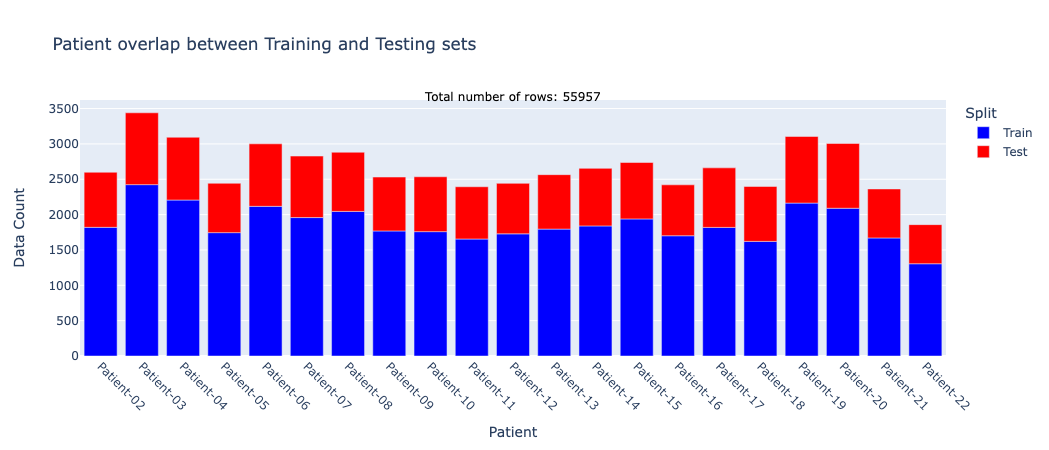
\includegraphics[width=1.0\textwidth]{../src/resources/bad_split.png}
                        \caption{
                            Visualization of the ineffective data splitting approach.
                        }
                        \label{fig:badsplit}
                    \end{figure}
        
                    \newpage

            \subsection{Effective} \label{sec:goodsplit}
            Data is split into training and testing sets based on the patient's unique ids. The patients are split into training and testing sets, and then the data is split based on the patient's unique ids.  The code snippet in \ref{lst:goodsplit} demonstrates this approach.

\begin{lstlisting}[
    caption={Effective approach to splitting the data into training and testing sets.}, 
    label={lst:goodsplit}]
    def split_data(data: pd.DataFrame) -> tuple:    
        # Patient's unique ids is extracted
        unique_patients = data['patient'].unique()

        # Patient's unique ids are split into training and testing sets
        train_patients, test_patients = train_test_split(unique_patients, test_size=0.3, random_state=42)

        # Training and testing sets are created
        train_data = data[data['patient'].isin(train_patients)]
        test_data = data[data['patient'].isin(test_patients)] 

        X_train = train_data.drop(columns=['label', 'patient'])
        y_train = train_data['label']

        X_test = test_data.drop(columns=['label', 'patient'])
        y_test = test_data['label']
        
        return X_train, X_test, y_train, y_test
\end{lstlisting}

            Figure \ref{fig:goodsplit} visualization demonstrates why this approach is effective. The data is split based on the patient's unique ids, so the model will be trained on data that it will not be tested on. This means that the model will be tested on unseen data, which is a good indicator of the model's performance.

            \begin{figure}[H]
                \centering
                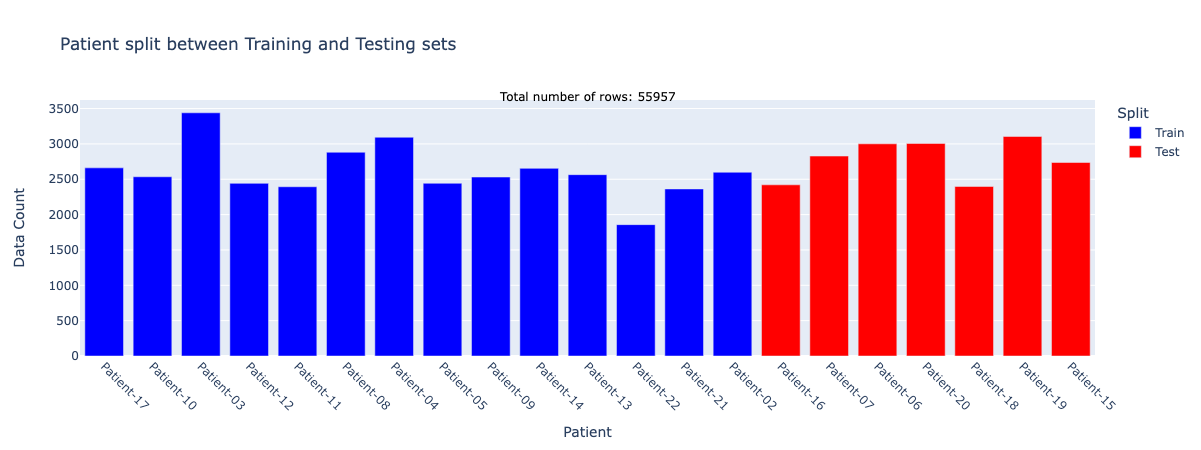
\includegraphics[width=1.0\textwidth]{../src/resources/good_split.png}
                \caption{
                    Visualization of the effective data splitting approach.
                }
                \label{fig:goodsplit}
            \end{figure}

    \newpage
        \subsection{Sequential} \label{sec:seqsplit}
            Data is split into training and testing sets based on the patient's unique ids, then the sets are split into sequences. Where each sequence represents the stack of frames that make up a movement. The code snippet in \ref{lst:seqsplit} demonstrates the splitting into sequences of the data. 

\begin{lstlisting}[
    caption={Effective approach to splitting the data into training and testing sets.}, 
    label={lst:seqsplit}]                
    def sequences(df: pd.DataFrame, feature_columns: list, sequence_column: str) -> tuple:
        sequences = []
        labels = []
        current_sequence = []
        current_check = None

        for _, row in df.iterrows():
            check = row[sequence_column]
            label = row['label']
            if check != current_check and current_sequence:
                sequences.append(np.array(current_sequence))
                labels.append(label)
                current_sequence = []
            current_sequence.append(row[feature_columns].to_numpy())
            current_check = check

        if current_sequence: 
            sequences.append(np.array(current_sequence))
            labels.append(label)

        return sequences, labels
\end{lstlisting}

            Figure \ref{fig:seqsplit} visualization shows how for each movement the data is split into sequences for training and testing. However, using only this approach is not enough, as the sequences are of different lengths due to each movement having a variable number of frames. This means that the sequences cannot be used as input for the models since they require a fixed input size. 
        
            \begin{figure}[H]
            \centering
            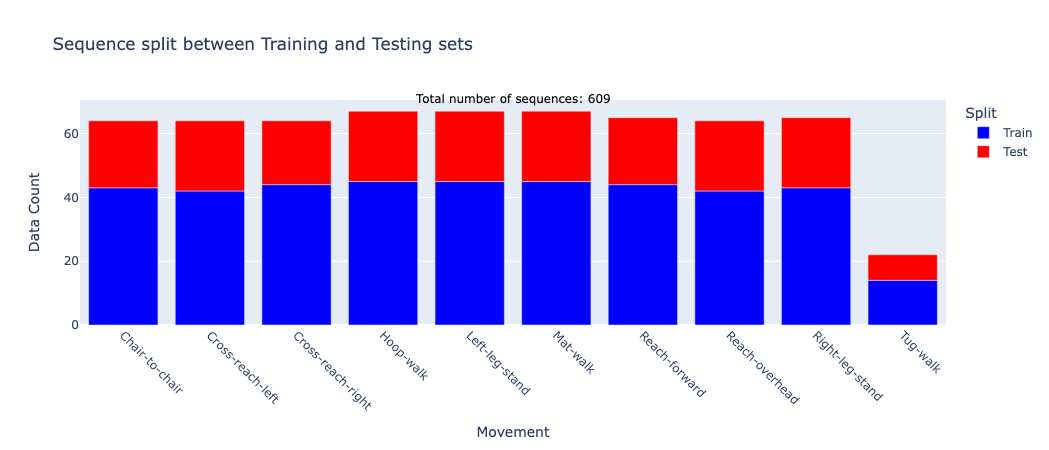
\includegraphics[width=1.0\textwidth]{../src/resources/seq_split.png}
            \caption{
                Visualization of the sequences splitting approach.
            }
            \label{fig:seqsplit}
        \end{figure}

        \newpage 

        To solve the variable length problem, the sequences are aggregate into a single featurere vector. The code snippet \ref{lst:seqagg} demonstrates this approach. In Figure \ref{fig:seqlength}, the length of the sequences before and after aggregation is visualized. The aggregation is done by calculating the mean of each feature for each frame in the sequence. This results in a single feature vector for each sequence, which can be used as input for the models.

\begin{lstlisting}[
    caption={Sequences are aggregated into a single feature vector.}, 
    label={lst:seqagg}]                
    def aggregate_features(sequences: list) -> np.ndarray:
            return np.array([np.mean(sequence, axis=0) if sequence.size != 0 else np.zeros(sequence.shape[1]) for sequence in sequences])
\end{lstlisting}
        
However, there are some drawbacks to this approach. The aggregation results in a loss of information, as the data is no longer represented as a sequence of frames. In addition, the aggregation results in a loss of the temporal information, as the order of the frames is lost. This means that the models will not be able to learn the temporal patterns in the data.

\begin{figure}[H]
    \centering
    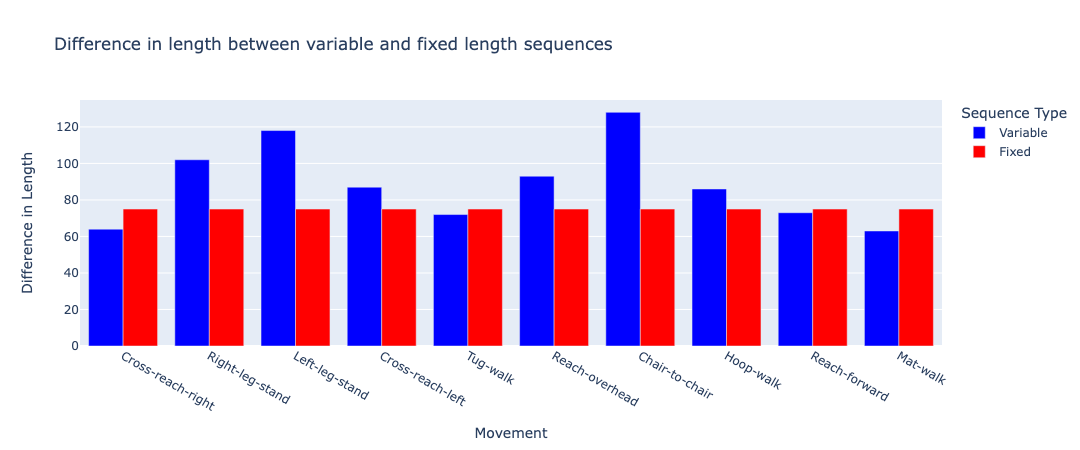
\includegraphics[width=1.0\textwidth]{../src/resources/plots/length.png}
    \caption{
        Visualization of the length of the sequences before and after aggregation.
    }
    \label{fig:seqlength}
\end{figure}

    \newpage
    
    \section{Feature Engineering} \label{sec:feature_engineering}
        Feature Engineering is the process of extracting features from raw data. In this thesis, the raw data is the Kinect Skeleton data, which is a series of 3D coordinates. The features extracted from the Kinect Skeleton data are presented in Table \ref{tab:features_table}.

        \subsection{Overview}
        \begin{table}[ht]
            \centering
            \begin{tabular}{@{}clcl@{}}
                \toprule
                \multicolumn{4}{c}{\textbf{Features}} \\
                \midrule
                1 & Duration & 2 & Area \\
                3 & Velocity & 4 & Distance \\
                5 & Displacement & 6 & Acceleration \\
                7 & Energy & 8 & Power  \\
                9 & Directional Changes & 10 & CoM Trajectory  \\
                11 & Peak Velocity  & 12 & Peak Acceleration  \\
                13 & Sway  & 14 & Vertical Displacement  \\
                15 & Forward Displacement & 16 & Jerk \\
                17 & Range of Motion \\
                \bottomrule
            \end{tabular}
            \caption{Features extracted from the Kinect Skeleton data.}
            \label{tab:features_table}
        \end{table}

        \subsection{Calculation Methods}
    %         The features presented in Table \ref{tab:movement_table} are calculated using the following methods. For each of the features, the formula used to calculate it is presented, along with a brief description.

    %         \subsubsection{Duration}
    %         The duration of a movement is defined as how long it takes for the movement to be performed from start to finish. It is calculated as the difference between the maximum and minimum datetime column values of the movement, as shown in Equation \ref{eq:duration}. The difference is calculated in seconds.
    %             \begin{equation}\label{eq:duration}
    %                 D = (\text{{max\_datetime}} - \text{{min\_datetime}})
    %             \end{equation}
    %         \subsubsection{Area}

    %         \subsubsection{Velocity}
    %             The velocity of a movement is defined as the rate of change of the displacement over time. It is calculated as the square root of the sum of the squared displacement over time difference for each axis, as shown in Equation \ref{eq:velocity}. 
    %             \begin{equation}\label{eq:velocity}
    %                 \text{velocity} = \sqrt{\left(\frac{\text{displacement}_x}{\text{time difference}}\right)^2 + \left(\frac{\text{displacement}_y}{\text{time difference}}\right)^2 + \left(\frac{\text{displacement}_z}{\text{time difference}}\right)^2}
    %             \end{equation}

    %         \subsubsection{Distance}
    %             \begin{equation}
    %             \text{distance} = \sqrt{(x_2 - x_1)^2 + (y_2 - y_1)^2 + (z_2 - z_1)^2}
    %             \end{equation}
                
    %         \subsubsection{Displacement}

    %         \subsubsection{Acceleration}

    %         \subsubsection{Energy}

    %         \subsubsection{Power}

    %         \subsubsection{Directional Changes}

    %         \subsubsection{CoM Trajectory}

    %         \subsubsection{Peak Velocity}

    %         \subsubsection{Peak Acceleration}

    %         A set of joints is defined as follows: \textit{AnkleLeft}, \textit{AnkleRight}, \textit{WristLeft}, \textit{WristRight}, \textit{SpineMid}. For each of these joints, the following features are calculated. 
            
    %         \subsubsection{Sway}
    %         \begin{equation}
    %             \text{Total Sway} = \sum_{t=1}^{n} \sqrt{(x_t - x_0)^2 + (y_t - y_0)^2 + (z_t - z_0)^2}
    %         \end{equation}

    %         \subsubsection{Vertical Displacement}
    %         \begin{equation}
    %             \text{Total Vertical Displacement} = \sum_{t=2}^{n} |y_t - y_{t-1}|
    %         \end{equation}

    %         \subsubsection{Forward Displacement}
    %         \begin{equation}
    %             \text{Total Forward Displacement} = \sum_{t=2}^{n} |z_t - z_{t-1}|
    %         \end{equation}
                
    %         \subsubsection{Jerk}
    %         \begin{equation}
    %             J_{\text{magnitude}}(t) = \sqrt{J_{x}(t)^{2} + J_{y}(t)^{2} + J_{z}(t)^{2}}
    %         \end{equation}
    %         \begin{equation}
    %             \text{Total Jerk} = \sum_{t=3}^{n} \sqrt{{(J_{x}(t))^2 + (J_{y}(t))^2 + (J_{z}(t))^2}}
    %         \end{equation}
                 

    %         \subsubsection{Range of Motion}
    %         The 
    %         \begin{equation}
    %             \text{Total ROM} = \sum_{i=1}^{n} \sqrt{(x_i - x_{i-1})^2 + (y_i - y_{i-1})^2 + (z_i - z_{i-1})^2}
    %         \end{equation}
                         
\cleardoublepage